
% .:: Laden der LaTeX4EI Formelsammlungsvorlage
\documentclass[fs, footer]{latex4ei}

\usepackage{listings}
% Dokumentbeginn
% ======================================================================
\begin{document}


% Aufteilung in Spalten
\begin{multicols*}{4}
\title{Network Security}


\section{Introduction}

	\sectionbox{
	\subsection{Security Trends}
	Network security is an issue since \emph{critical infrastructures} in the open systems with a growing user base (\ra \emph{increasing risk}) are threatend by \emph{organized crime}.
	}
	\sectionbox{
	\subsection{Security Threats}
	\textbf{Asymmetric Threat:} Defenders must protect against all exploits on all systems but attackers can attack only a few.

	\textbf{Attacker Motivation:} Ego, Revenge, Destruction, Criminal intend, Aquisition of resources, Acquistion of sensitive information
	}
	\sectionbox{
	\subsection{Security concepts}
	\textbf{CIA Triad}
	\begin{itemize}
	 	\item Confidentiality (prevention of unauthorized disclosure)
	 	\item Integrity (prevention of unauthorized modification or deletion)
	 	\item Availability (prevention of unauthorized withholding)
	 \end{itemize}

	 Also: Authenticity, Accountability, Non-repudiation (Nichtabstreitbarkeit), Privacy

	 (Classification by Steve Kent)
	 \textbf{Passive attacks:} Confidentiality (Content compromise, Traffic analysis)

	 \textbf{Active attacks:} Availabilty (Denial of service), Integrity and Authenticity (Modification, Replay, Fabrication)

	 \textbf{Secure Channel:} secure = authentic (of the sender) and confidential (no eavesdropping)

	 \textbf{Security on OSI-Layers:} Physical (Link encryption), Network (IPSEC), Transport (SSL), Application (SSH)

	 }


\section{(In)securtity, Risk and the Lifecycle of Vulnerablities}


	\sectionbox{
	\subsection{(In)security Landscape}
	General: complexity is bad (but increases fast)

	Security of a system := Security of its weakest link
	}
	\sectionbox{
	\subsection{Vulnerablity Lifecycle}

	\textbf{Security vulnerability} \\
	a weakness in a system allowing an attacker to violate the confidentiality, integrity, availability of the system or the data and applications it hosts

	disagreement on what is a vulnerability possible (it's a a feature not a vulnerability)

	\textbf{CVE}
	Standard names for all publicly known vulnerabilities and security exposures. De facto standard.

	Form: \emph{CVE-Year-AnyDigits}

	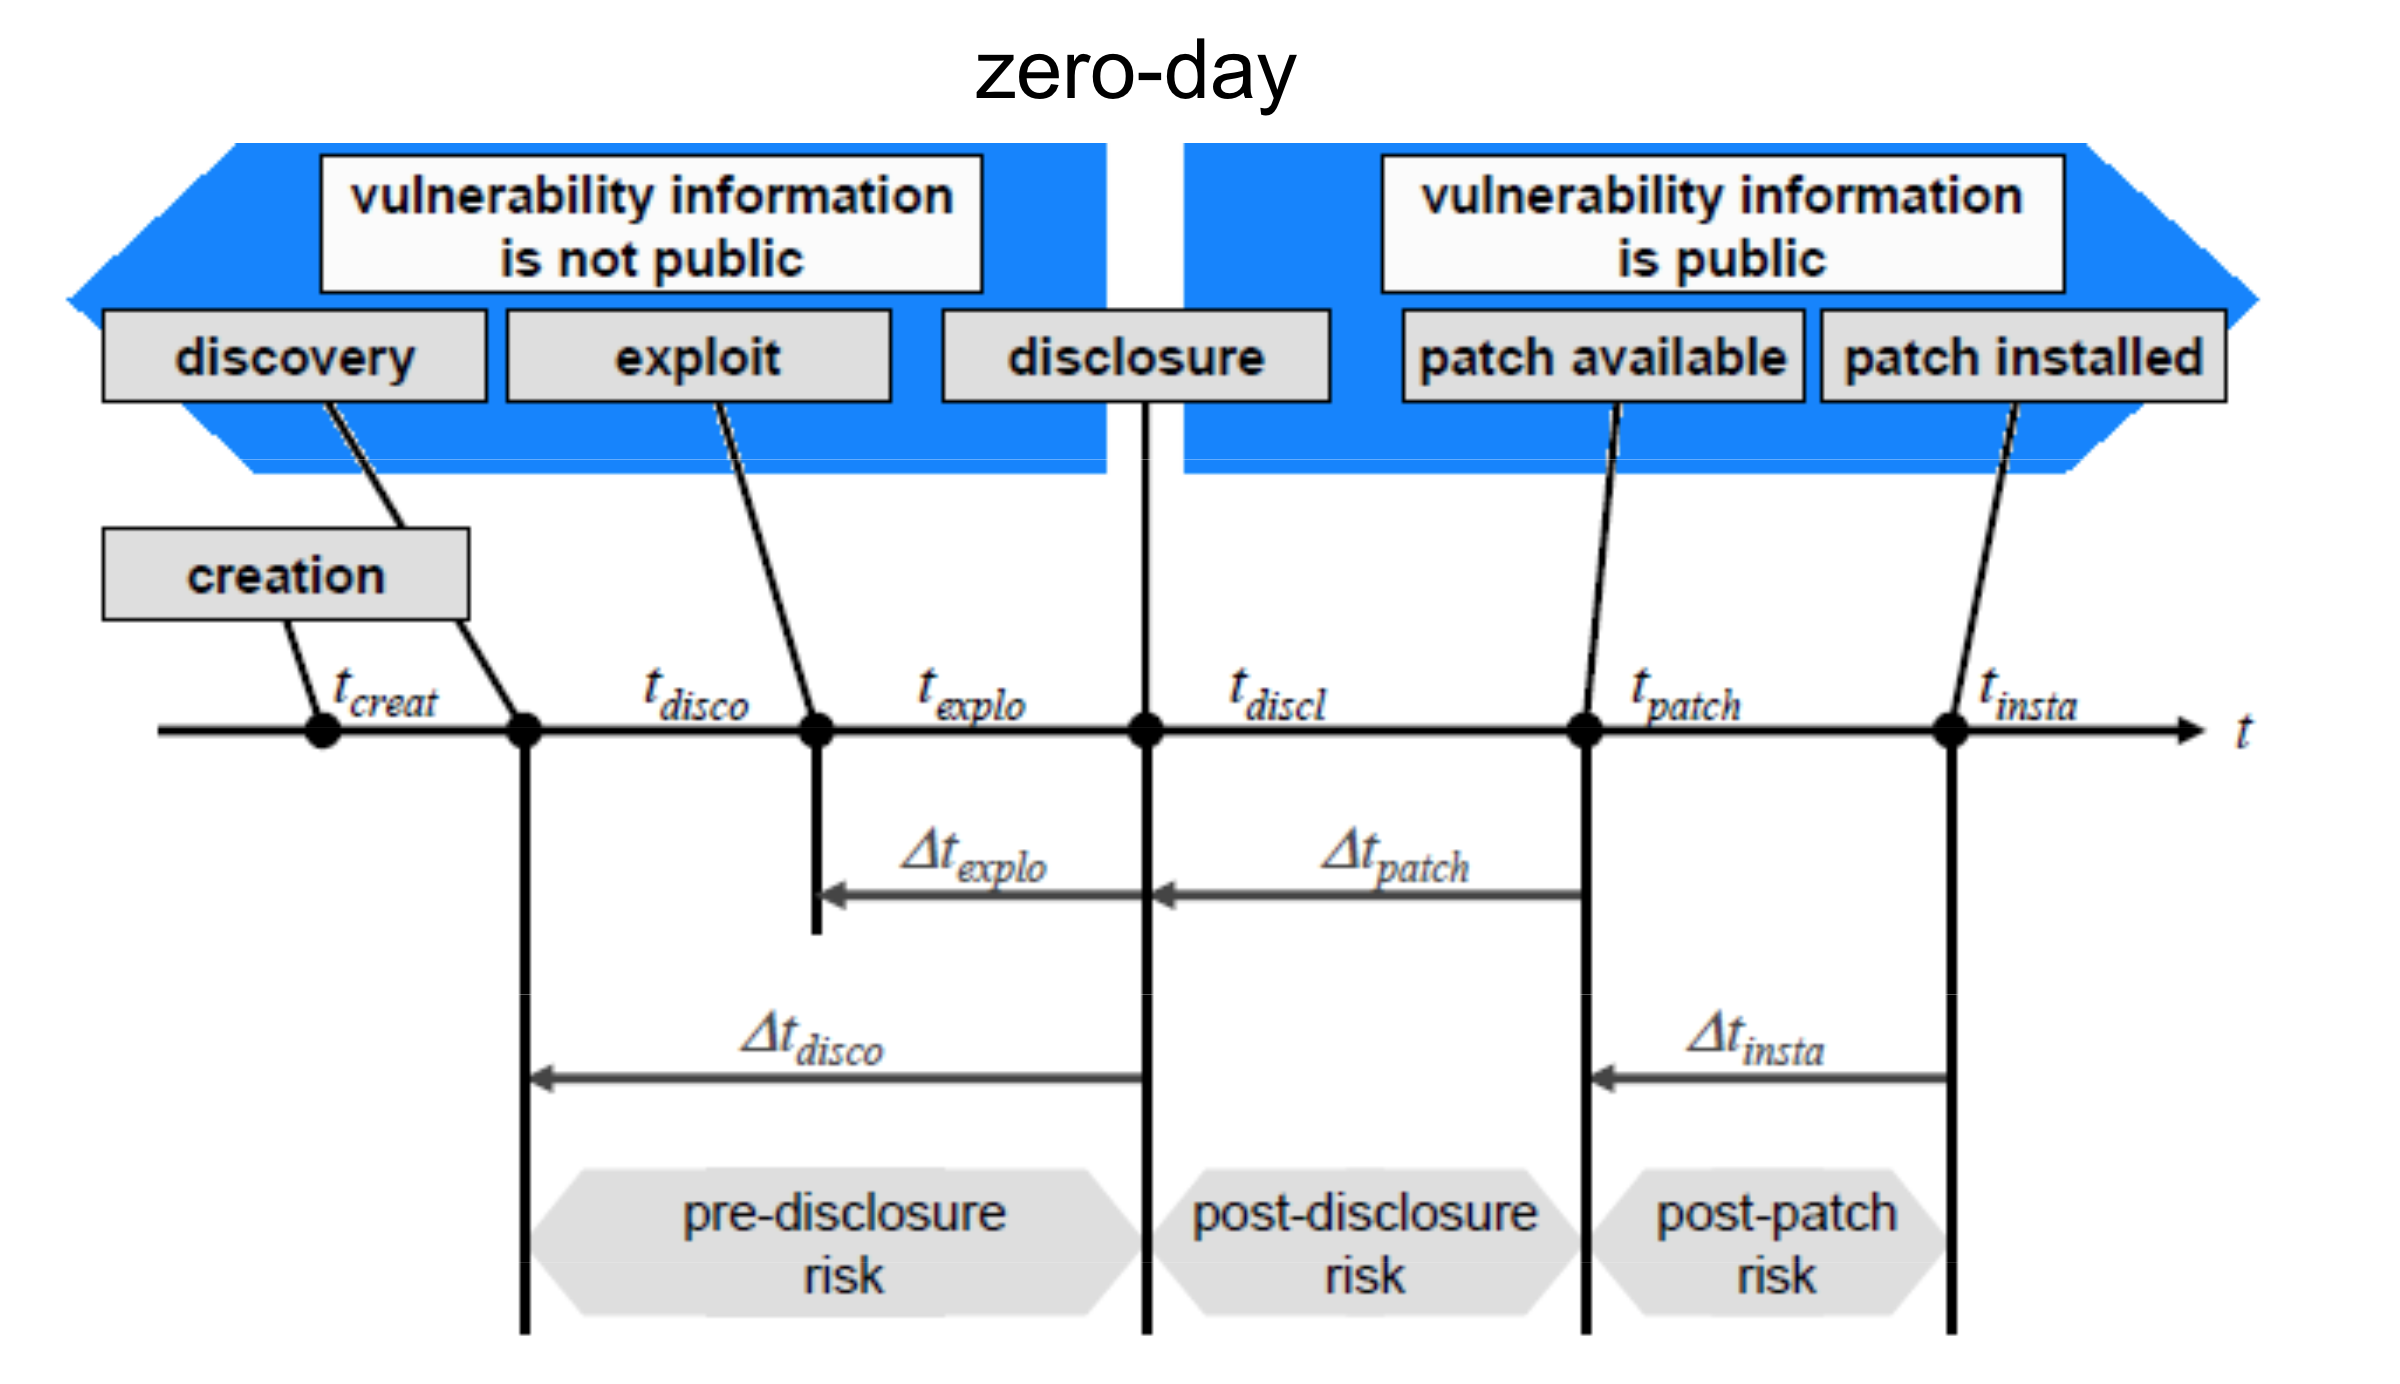
\includegraphics[width=\columnwidth]{img/VUL-LC.png}


	\textbf{Numbers:}\\
	50 \% of vulnerabilities known to insiders 30 or more days before disclosure (less-than-zero-day)

	At disclosure:  $\approx 50 \%$ unpatched

	A month after disclosure: $\approx 50 \%$ unpatched \\

	\textbf{Zero-day} Date when the vulnerability becomes known by the public

	\textbf{Zero-day-exploit} Attack that exploits a previously unknown vulnerability
	}
	\sectionbox{
	\subsection{Dynamics of (In) Security}
	\begin{itemize}
		\item extremely high dynamics around the disclosure
		\item exploit availability stays higher than the patch availability
		\item insiders: may know undisclosed vulnerabilites
	\end{itemize}

	\textbf{Gap of insecurity:} Difference between the exploit and patch (the bad a consistently faster than the good)

	}

	\sectionbox{
	\subsection{Risk}
	There is such thing as absolute security

	Trade-Off between security and financial, social, functional, \ldots

	\subsubsection{Risk analysis}
	\begin{itemize}
		\item What assets are we trying to protect?
		\item what are the risk to those assets?
		\item How well does the security solution mitigate those risks?
		\item What other risks does the security solution cause?
		\item What costs and trade-offs does the security solution impose?
	\end{itemize}
	\ra is the trade-off worth if?

	\subsubsection{Risk management}
	Security is relative \Ra manage risks

	Options: avoid, decrease, transfer, accept risk

	Business sense: risk $<$ opportunity
	}


\section{Identity and Authentication}
\sectionbox{
	\subsection{Identity and Identity Theft}

	\textbf{Identity:} An identity specifies a principal (a unique entity)

	e.g. Individuals, Physical objects, Logical objects, Groups

	\textbf{Identitfy theft:} Identity theft is a crime in which imposters obtain key pieces of personally identifying information and use them for their own personal gain or to do harm

	Variants: Financial, Criminal, Identity cloning, Business

	(12.6 million US-citizens in 2012 with 4.6 billion total damage)
	}
\sectionbox{
	\subsection{Authentication}

	\textbf{Authentication:} Authentication is the process of verifying an identity claim of an entity. It binds the principal to an identity

	\textbf{Criteria:}
	\begin{itemize}
		\item Something an entity knows (e.g. password, PIN)
		\item Something an entity has (e.g. key, card)
		\item Something an entity is (e.g. biometric characteristic)
		\item rarely used: location, ability
	\end{itemize}

	\textbf{Weak authentication:} checking only one authentication criteria

	\textbf{Strong authentication:} checking two or more authentication criteria
}

	\subsection{Authentication Protocols}
\sectionbox{
	\subsubsection{OpenID}

	Standard for decentralised user authentication:
	use existing account to sign in to multiple websites without creating a new password

	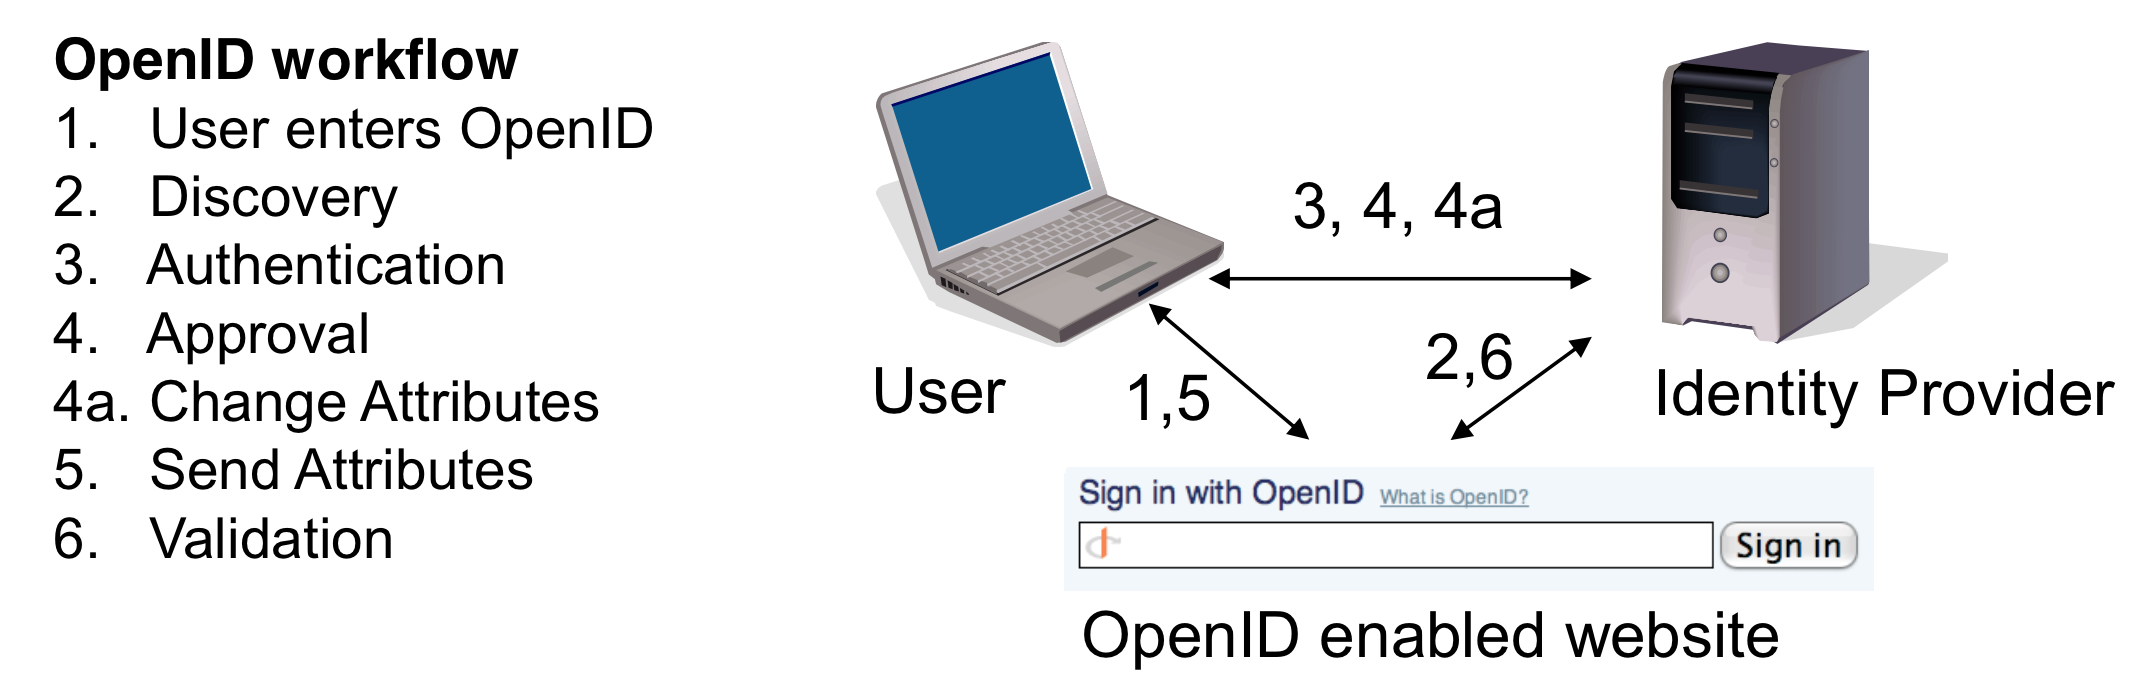
\includegraphics[width=\columnwidth]{img/OpenID.png}
}
\sectionbox{
	\subsubsection{OAuth}
	A web user (resource owner) grants a
	printing service (client) access to her protected photos stored at a photo sharing service (resource server), without sharing her username and password with the printing service.
	Instead, she authenticates directly with a server trusted by the photo sharing service (authorization server) which issues the printing service delegation-specific credentials (access token).

	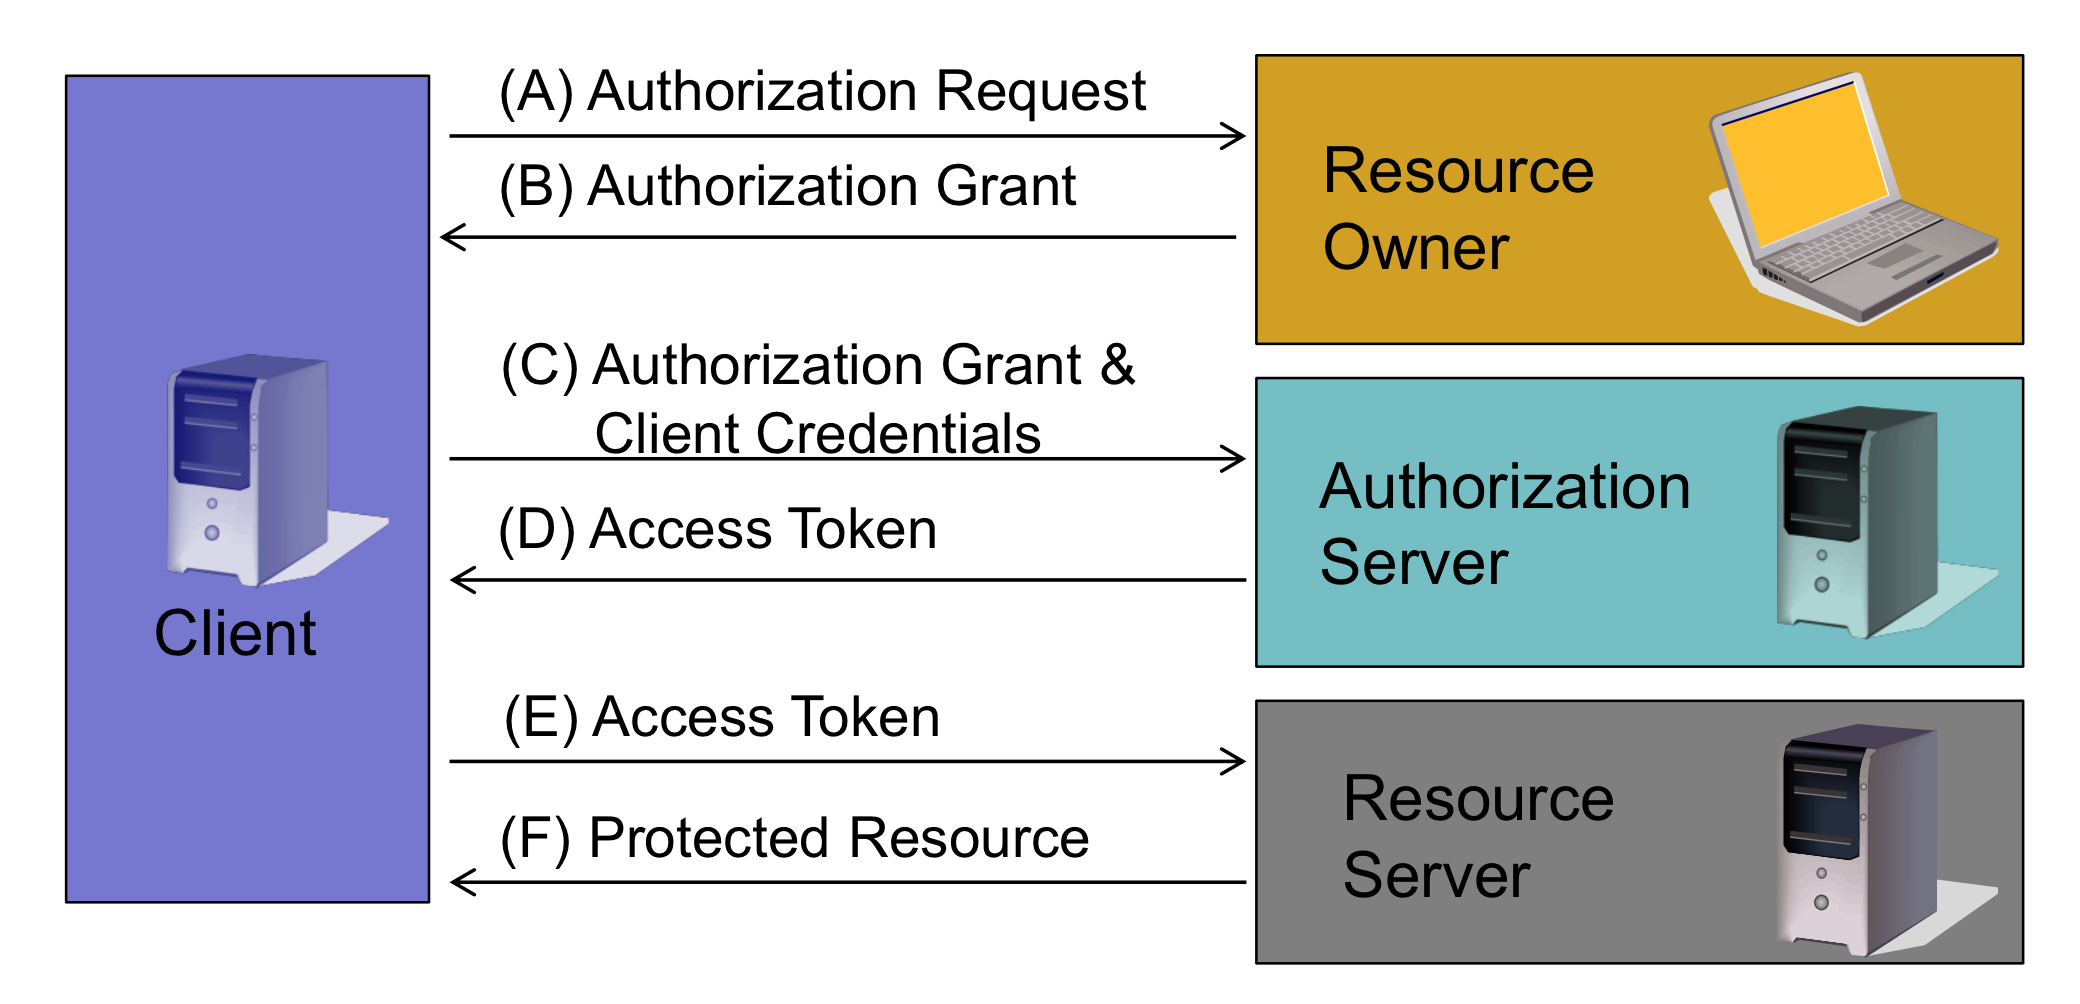
\includegraphics[width=\columnwidth]{img/OAuth.png}

	(A) Client requests authorisation from the resource owner or authorization server. \\
	(B) Client receives an authorisation grant by the resource owner. Authorization grant type depends on the method used by the client and supported by the authorisation server to obtain it. \\
	(C) Client requests an access token by authenticating with the authorization server using its client credentials (prearranged between the client and authorization server) and presenting the authorization grant. \\
	(D) Authorisation server validates  client credentials and the authorization grant, and if valid issues an access token.\\
	(E) Client requests protected resource from the resource server. Authentication by access token.\\
	(F) Resource server validates the access token \ra valid \ra serves request\\
}
\sectionbox{
	\subsubsection{3D Secure}
	A protocol used widely to authenticate online card transactions.

	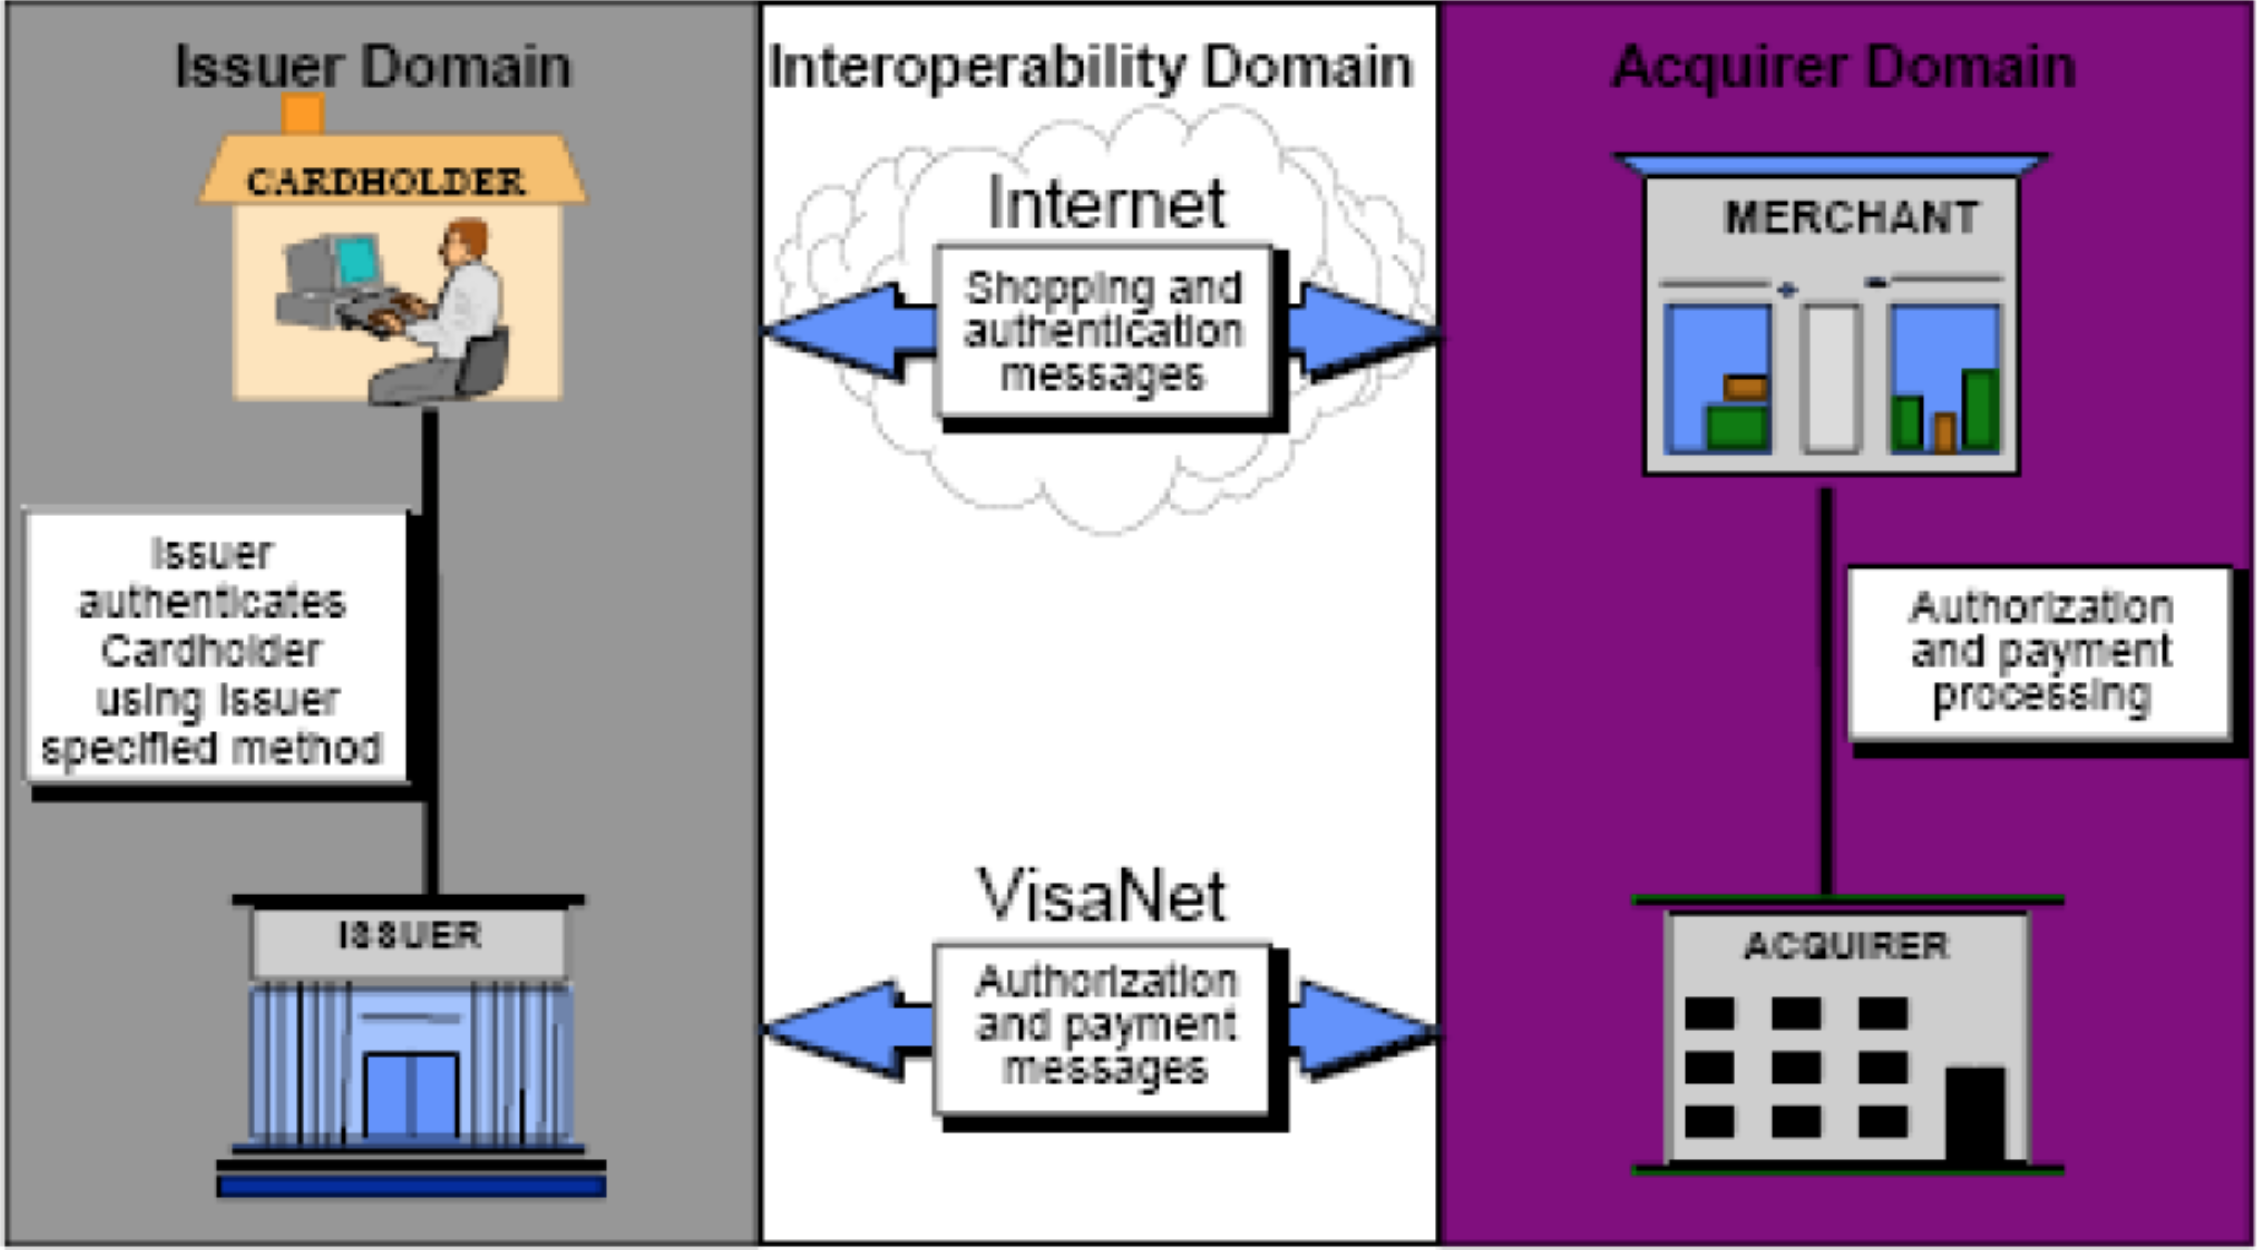
\includegraphics[width=\columnwidth]{img/3DSecure.png}
	After entering payment card details on merchant site:
	\begin{itemize}
	\item 3D Secure pops up a password entry form to a bank customer
	\item customer enters a password and, if it was correct,
	\item customer is returned to the merchant website to complete the
	transaction and
	\item the merchant gets an authorisation code to submit to his bank
	\end{itemize}

	\textbf{Problems:} Pop-Up blockers, Activation during shopping, SLL verification not visible, liability shift, weak bank authentication, no password reset procedure, privacy issues\\
}
\sectionbox{

	\subsubsection{802.1x}
	Client-server based access control protocol that restricts unauthorised devices from connecting to a (W)LAN through publicly accessible ports

	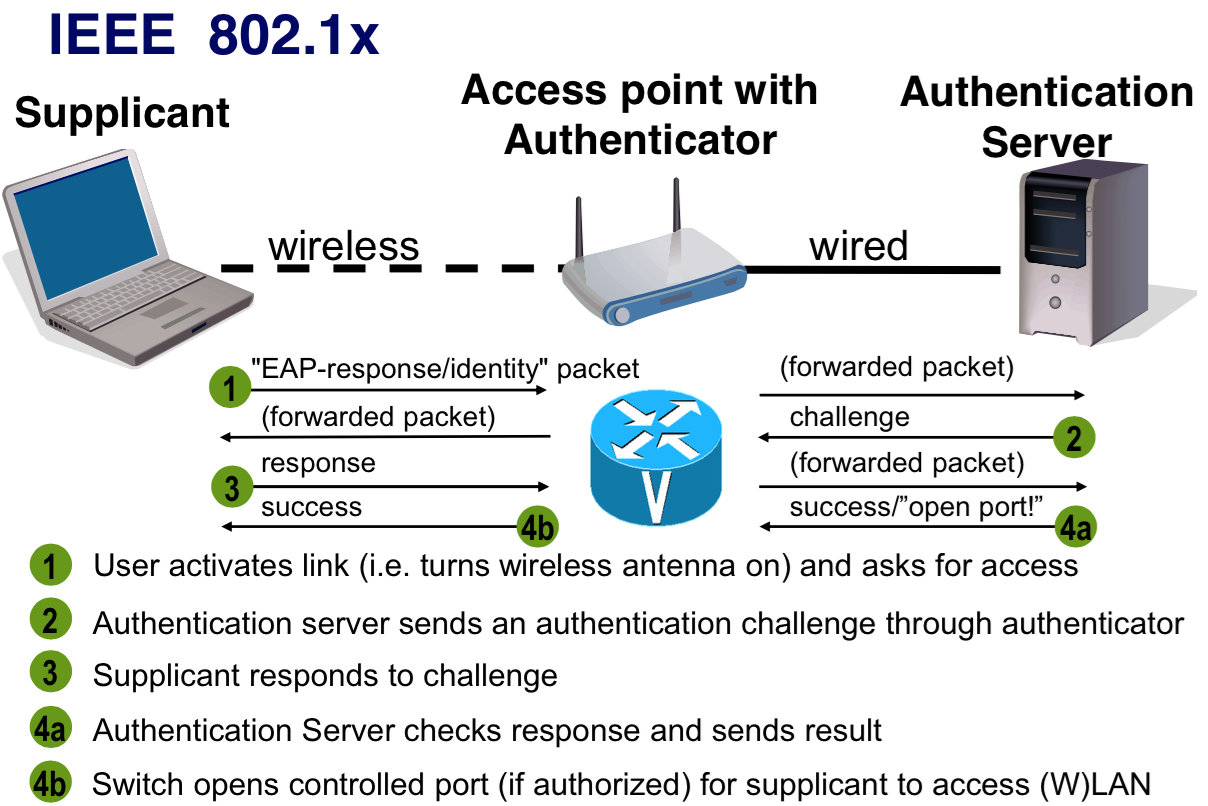
\includegraphics[width=\columnwidth]{img/8021x.png}

	\textbf{EAP} (Extensible Authentication Protocol): Authentication framework on the data link layer supporting multiple methods (MD5, OTP, TLS, TTLS) without requiring an IP.

	\textbf{Identity and Security}: Authentication (Who?) , Authorisation (What?) , Access Control, Policy enforcement

	\textbf{Benefits:} Standard based technology, control at link layer, interoperating wifi and wired, centralised user administration

	\textbf{Drawbacks:} Authenticator authentication, Man-in-the-middle, session hijacking
}

\sectionbox{
	\subsection{Anonymization}

	\textbf{Levels of Anonymity:} Identity (principal known), Pseudonymity (indirectly kown as pseudonym), anonymity (part of anonymity set but within no distinguishing)

	\textbf{Pseudonyms:} public (\ra identification), non-public (\ra pseudonymity), unlinkable (\ra anonymity)

	\textbf{Use cases:} \\
	physical: feedback, voting, whistleblowing, censorship \\
	digital: digital cash, digital voting, illegal activities

	\textbf{Oninon routing: } Data is encapsulated multiple times and only the next hop is known to each node

	\textbf{Mixnet:} proxy handles messages in batches (transformed and premutated) \Ra unlinkablity of incoming and outgoing messages

	\textbf{Attacks:} Traceback (break systems on path), Collusion (bad nodes), Traffic analysis (tagging with bit errors, replay messages - defense: heartbeats, traffic shaping, padding) , Logging (???)
}

\section{Firewalls, IDS and NAT Traversal}
\sectionbox{
\subsection{Firewalls}
Hardware or software device which is configured to permit, deny or proxy data through a computer network with different levels of trust. The configuration is called \emph{policy}.

\textbf{Types:} simple packet filter, stateful filter, application layer proxy

\textbf{Rules:} Filtering (outgoing, incoming), Default (accept, reject), Deny (Drop, Reject), Addressing Transparency (firewall and network fingerprinting)

\subsubsection{Stateless Firewall}
Functionality: examine on network layer, decision based on header

Pro: application independent, good performance

Cons: no state or application context

\subsubsection{Stateful Firewall}
keeps track of state. Decision based on \emph{session state}

Pro: more powerful

Cons: no state for UDP, host vs. firewall state, state explosion

 \subsubsection{Application Layer Firewall}
 take application state into account

 Pro: application aware

 Cons: many application protocols, performance

 \subsubsection{Web Application Firewall}
protects web-based applications from malicious requests (often reverse proxy)

Filtering: signatures, black/whitelisting

 \subsubsection{Firewall Attack techniques}
 \begin{itemize}
 	\item IP source spoofing
 	\item artificial fragmentation
 	\item vulnerabilites
 	\item Denial of Service (state explosion)
 	\item Tunneling/Covert channel (ICMP, DNS, \ldots)
 \end{itemize}

 \subsubsection{Firewall detection}

 Port scanning: traceroute, src IP of response

 TTL:  let expire TTL one hop past firewall

 \subsubsection{Oranizational challenges}
 \begin{itemize}
  	\item Large rulesets
  	\item Big Organizations
  	\item Conflict: Networking vs. security staff
  \end{itemize}

  \subsubsection{IP Tables}
	Netfilter rule:
	iptables -A INPUT -i eth0 -m state --state ESTABLISHED, RELATED -j ACCEPT

	Iptables rule:  iptables -A INPUT -p tcp -s 0/0 -d 0/0 --destination-port 80 --syn -j ACCEPT

	\subsubsection{NAT (Network Address Translation)}
	One way to the Internet (multiple hosts on private network using the same public IP address). IP Address rewriting.

	Benefits: Prevents malicous activity from outside, saves address space

	Drawbacks: no end-to-end connectivity, some protocols don't work

	\subsubsection{NAT UDP Hole Punching}

	$\Ra$ exam relevant?
}
\sectionbox{
\subsection{Intrustion Detection and Prevention Systems}
try to detect intrusions on the network by comparing to attack signatures. Block traffic after detection.

\subsubsection{Classification}
\textbf{Object of observation:}

Packet:

Flow: scalabilty (+), encryption (+), not content-based (-)

\textbf{Point of observation:}

Host: hard deployment (-), context information (+), one sensore per machine (+)

Network: easy deployment (+), multiple machines (+), unknown machines(-), preformance (-)

\textbf{Method of observation:}

Signature: precision (+), not detecting unknown attacks (-)

Behavior: unknown attacks (+), difficult to find ground truth (-), false positives (-)

\subsubsection{Challenges}
\begin{itemize}
 	\item false alarms
 	\item high network speeds
 	\item sensor management and signature distribution
 	\item policy management
 	\item manpower
 \end{itemize}

 \subsubsection{Attacks}
 \begin{itemize}
 	\item Flooding / resource exhaustion
 	\item algorithmic Complexity Attacks (e.g. on hash table)

 \end{itemize}
}

\section{The Domain Name System Security}
\sectionbox{
\subsection{DNS}
\emphbox{DNS is a global, distributed, robust system for name to IP address resolution}

DNS is the glue of the internet: Nearly all activities start with a DNS lookup

Orgiginally: no security considerations

Design:
\begin{itemize}
	\item Client-Server application
	\item Hierarchical System
\end{itemize}

\textbf{Zone:} Collection of hostnames/IP pairs managed together

\textbf{Nameserver (authoritative): } Server that answers DNS queries (Responsible DNS Server for each zone)

\textbf{Resolver:} Client part of DNS that resolves domain names

\textbf{Recursive name server:}  Answers queries for all zones

\textbf{Stub resolver:} Forwards request to recursive name server (typically used by end-hosts)

\textbf{Caching:} Reduces overhead. Lifetime controlled by TTL
}
\sectionbox{
\subsection{Attacks on DNS}

\subsubsection{Denial of Service on DNS}
Tageting the 13 DNS root servers which are a bottleneck resource. However overprovisioning (13 clusters) prevents most attacks.

\subsubsection{Account-Takeover}
Attacking the web interfaces of registrars and try to enter malicious name servers.

\subsubsection{Manipulate local DNS settings}
\begin{itemize}
	\item Manipulate local host configurations (access to the local machine nescessary)
	\item Spoof DHCP replies (access to LAN nescessary) \ra countermeasure: authentification for DHCP messages
	\item Set up Malicious DHCP server that is faster than the vaild one
\end{itemize}

\subsubsection{Manipulate DNS lookup process}

\textbf{Bailiwick Checking:} Is the server authorized to respond to DNS requests for the domain.

\textbf{Weak authentication:} Port, TXID, Query string - first good answer wins

3 possible answers to DNS queries:
\begin{itemize}
   	\item Here is your answer
   	\item go away
   	\item I don't know ask \ldots
\end{itemize}


\subsubsection{The Kaminsky Attack}
\begin{itemize}
	\item Inject query on the client Random.www.bank.com
	\item reply multiple times  (TXID 0-200)
	\item Send name server redirections
\end{itemize}
$\Ra$ Fix: Source Port Randomization. Chance: $65536 \cdot (65536 - 1024)$ to 1
}

\sectionbox{
\subsection{DNSSEC}
Provides:
\begin{itemize}
	\item Authenticity
	\item Integrity
	\item Backward compatibility
\end{itemize}

Drawbacks
\begin{itemize}
	\item No confidentiality
	\item No protection against DoS
\end{itemize}

All records are signed: Key pairs for each zone $\ra$ Integrity

Chain of trust $\ra$ Authenticity
}

\section{Availability and Denial of Service}

\section{Secure Channels: Principles, VPN, SSH}

\subsection{Security by Layer of the TCP/IP Model}
Properties of a secure channel: secure = authentic and confidential

\subsubsection{Security at Link Layer}
\begin{itemize}
	\item All traffic over a specific Link
	\item Often implemented in hardware
\end{itemize}

Pro: Speed, Seamless

Drawbacks: every link seperately, trust in link operator

\subsubsection{Security at Internet Layer}

\subsubsection{Security at Transport Layer}

\subsubsection{Security at Application Layer}

\subsection{VPN}

\subsection{SSH}

% Network layers (and security in different layers)
% VPN technologies (bluilding blocks, IPSec)
% SSH (algorithms parameters)
% Passwords

\section{TLS}

\section{Crypto-Refresher}

\section{Web Application Security: Session State}

\section{Web Application Security: SQL Injection}

\section{Cross-Site Scripting (XSS)}
\subsection{Same-origin policy}
A script can only access content and properties of a document loaded from the same origin.
\begin{itemize}
  \item same protocol
  \item same hostname
  \item same port
\end{itemize}
URL path is ignored for the same-origin policy

\textbf{Interaction of different origins}
\begin{itemize}
  \item Link
  \item Iframe: Shown inside me.tld but cannot exit iframe
  \item POST: POSTing data to you.tld
  \item script include: Evaluted in context of me.tld ($\ra$ dangerous)
  \item Asynchronous Requests (AJAX): Different origin only possible if allowed by target domain (with Access-Control-Allow-Origin Header)
\end{itemize}

\subsection{Cross-Site Scripting (XSS) Attacks}
XSS flaws occur whenever a web app takes user supplied data and sends it to the browser without first \emph{validating} or \emph{encoding} the content.

\textbf{Target:} The user of the app insted of the app itself

\textbf{Infection path:} email, chat, uploaded files \ldots

\textbf{Dangerous content:} advertisments, user contributed content, widgets (counters, scripts \ldots)

\subsection{XSS prevention}
\begin{itemize}
  \item test your web app
  \item input sanitization (check user submitted content)
  \item HTML output encoding
\end{itemize}

\subsection{Data Leakage Attack}
Attacker includes script that reads session cookies and sends them to an evil server. $\ra$ Solution: HTTPOnly cookies

\subsection{Request Forgery (XSRF)}
A form form one domain posts a request to a different domain through an authenticated session.

\begin{itemize}
  \item write-only attack
\end{itemize}

\textbf{Solution:} CSRF Token, ask for password, check HTTP referer, show captcha

\subsection{Script inclusion (XSSI)}

\emph{Never include a script you do not trust!}

Data is retrieved from the web server with a request on the API endpoint. The browser automatically sends cookie and the JavaScript function in the evil website is called with the AJAX return data.

\textbf{Countermeasures:} security tokens derived from the cookie and a server challenge, use only HTTP POST, check HTTP referer

\section{Malware}

\section{Botnets + Malware Development and Demo}
Objectives:
	\begin{itemize}
		\item Buildup efficient infection and spreading
		\item prevent detection and removal
		\item address changing functionality needs
		\item handle large number of machines
		\item to business and technology challenges
		\item Anonymity prevent identification of operator
	\end{itemize}

Exploitation Phases:
	\begin{itemize}
		\item ID Theft
		\item Peer and Social Attacks (Trust misuse)
		\item Local Attacks (Local Network, USB)
		\item Attack Support (Host of Phising Site)
		\item External/Noisy Attacks (Scanning, Spam, DDoS)
	\end{itemize}

Fluxing Technologies:
\begin{itemize}
	\item IP-Flux: Constant change of IP address information related to a particular fully-qualified domain name (FQDN)
	\item Domain Flux: Constant change and allocation of multiple fully-qualified domain names (FQDN)
	\item Single-Flux: The FQDN of the CnC’s host has multiple IP addresses assigned (DNS A record)
	\item Double-Flux: The name servers of the CnC’s FQDN as well as the FQDN of the CnC’s host have multiple IP addresses assigned (DNS A and NS records)
\end{itemize}

Malware Development Process:
\\Develop, Crypt, Protect, Pack, Bind, QA

\section{Security Ecosystem and Detection Failures}

\section{E-Mail Spam}
\subsection{Define Spam}
\textbf{UCE}: Unsolicited Commercial Email

\textbf{UBE}: Unsolicited Bulk Email (not nescessaryliy commercial)
% Ende der Spalten

How Realtime Blacklists Lists Differ:
\begin{itemize}
	\item Nomination (how to get on the list)
	\item Listing lifetime (how to get off the list)
	\item Cost
	\item Operator
	\item Goal
\end{itemize}

Email Auth:
\begin{itemize}
	\item DomainKeys Identified Mail (DKIM): Pub/Priv Key Signing; pubkey distributed via DNS
	\item Sender Policy Framework: Domain owners publish list of IPs that are authorized
	\item SenderID: Match PRA domain against source IP via DNS (PRA is often From: header)
	\end{itemize}
	
\section{Guest Lectures}
DMZ: Compromised hosts in DMZ are no danger for internal network e.g.:(external - webserver(dmz) - database(internal))


\end{multicols*}

% Dokumentende
% ======================================================================
\end{document}

% ToDos:
